\tikzset{>=latex} % for LaTeX arrow head
\contourlength{1.6pt}
\colorlet{Bcol}{violet!90}
\colorlet{BFcol}{red!60!black}
\colorlet{Scol}{green!60!black}
\colorlet{veccol}{green!45!black}
\colorlet{Icol}{blue!70!black}
\colorlet{mucol}{red!90!black}
\tikzstyle{BField}=[->,thick,Bcol]
\tikzstyle{current}=[->,Icol] %thick,
\tikzstyle{force}=[->,thick,BFcol]
\tikzstyle{vector}=[->,thick,veccol]
\tikzstyle{mu vector}=[->,thick,mucol]
\tikzstyle{spin}=[->,very thick,Scol]
\tikzstyle{velocity}=[->,very thick,vcol]
\tikzstyle{charge+}=[very thin,draw=black,top color=red!50,bottom color=red!90!black,shading angle=20,circle,inner sep=0.5]
\tikzstyle{charge-}=[very thin,draw=black,top color=blue!50,bottom color=blue!80,shading angle=20,circle,inner sep=0.5]
\tikzstyle{metal}=[top color=black!15,bottom color=black!25,middle color=black!5,shading angle=10]
\tikzset{
  BFieldLine/.style={thick,Bcol,decoration={markings,mark=at position #1 with {\arrow{latex}}},
                                 postaction={decorate}},
  BFieldLine/.default=0.5,
  pics/magnet/.style={ %args={#1}
    code={
      \def\h{0.9}
      \coordinate (-N) at (0,\h);
      \coordinate (-S) at (0,-\h);
      \draw[pic actions,thick,top color=red!60,bottom color=red!90,shading angle=20]
        (-0.8*\h/2,0) rectangle ++(0.8*\h,\h);
      \draw[pic actions,thick,top color=blue!60,bottom color=blue!90,shading angle=20]
        (-0.8*\h/2,0) rectangle ++(0.8*\h,-\h);
      \node[pic actions] at (0, \h/2) {\textbf{N}};
      \node[pic actions] at (0,-\h/2) {\textbf{S}};
  }},
}

% B FIELD through current loop




% LARMOR PRECESSION


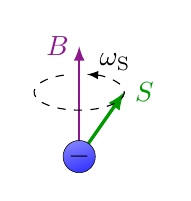
\begin{tikzpicture}
  \def\ang{55}
  \def\S{1.0}
  \def\B{1.4}
  \def\Rx{\S*cos(\ang)}
  \def\Ry{0.4*\Rx}
  \coordinate (O) at (0,0);
  
  \draw[BField] (O) -- (90:\B) node[left] {$\vb{B}$};
  \draw[spin] (O) -- (\ang:\S) node[right] {$\vb{S}$};
  \node[charge-,scale=1] (O) {$-$};
  \draw[->,dashed]
    (0,{\S*sin(\ang)})++(110:{\Rx} and {\Ry}) arc (110:440:{\Rx} and {\Ry})
    node[right=3,above right=-2] {$\omega_\mathrm{S}$};
  
\end{tikzpicture}
